\chapter{Giới thiệu}
\label{sec:gioithieu}


Chương này nhằm mục đích giới thiệu về bài toán sẽ được giải quyết trong luận văn và các khái niệm liên quan. Đầu chương sẽ nói về kỹ thuật dịch ngược, các ứng dụng của nó và những khó khăn trong quá trình dịch ngược. Phần tiếp theo trình bày bài toán đặt ra và các thách thức khi giải quyết bài toán. Phần cuối cùng tóm tắt cấu trúc của luận văn.

\section{Kỹ thuật dịch ngược và ứng dụng}
Trong khi kỹ thuật dịch phổ biến hiện nay là dịch từ mã viết bằng ngôn ngữ cấp cao xuống mã ngôn ngữ cấp thấp hơn, kỹ thuật dịch ngược thực hiện dịch từ mã ngôn ngữ cấp thấp lên mã ngôn ngữ cấp cao hơn. Kỹ thuật dịch ngược được sử dụng rất nhiều để hỗ trợ trong quá trình phát triển và sử dụng phần mềm:

\begin{itemize}
	\item Vì một lý do nào đó, mã nguồn của một phần mềm bị mất đi. Để tiếp tục phát triển phần mềm hoặc bảo trì phần mềm đó, ta cần phải khôi phục lại mã nguồn. Nếu viết lại một chương trình mới hoàn toàn từ các tài liệu sẵn có sẽ rất mất thời gian và không đảm bảo sẽ tương đương được phần mềm cũ. Vì vậy một giải pháp phổ biến hiện nay là dựa vào file thực thi dịch ngược lại và hiệu chỉnh để có được mã nguồn mới hoàn chỉnh.
	\item Các phần mềm độc hại như virus, malware thường sẽ được giấu kín mã nguồn, nếu có được mã nguồn của chúng thì việc tìm ra phương pháp giải trừ sẽ rất dễ dàng. Ta có thể ứng dụng kỹ thuật dịch ngược để làm việc đó.
	\item Chuyển đổi chương trình chạy trên một phần cứng này sang chương trình chạy trên một phần cứng khác. Ví dụ: ta có mã đang chạy trên chip 8051, nhưng vì chip sẽ bị ngừng sản xuất trong một vài năm nữa, nên yêu cầu đề ra là tạo ra mã tương đương chạy trên một con chip khác hiện đại hơn. Để làm được điều đó, ta có thể dùng trình dịch ngược dịch mã viết cho 8051 lên một ngôn ngữ cấp cao, và sử dụng tiếp trình biên dịch để dịch mã nguồn đó thành mã của chip thay thế. Vì mã viết trong các hệ thống nhúng thường là mã assembly, nên cụ thể trình dịch ngược trong hệ thống chuyển đổi này sẽ chuyển từ mã assembly lên mã ngôn ngữ cấp cao. Và đó cũng là đối tượng nghiên cứu của luận văn này.
	
	\begin{figure}[h]
		\centering
		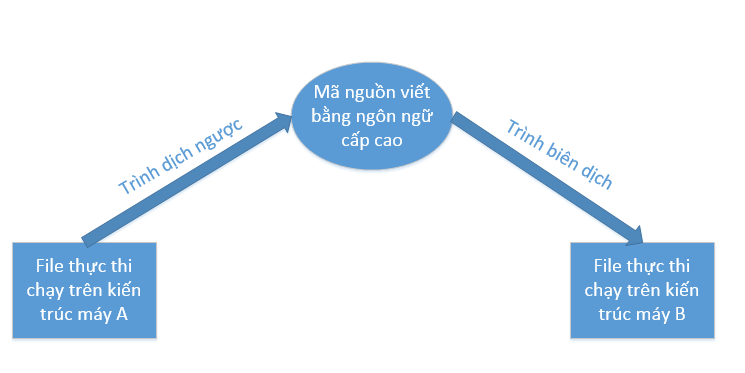
\includegraphics{fig12.png}
		\caption{Một ứng dụng của trình dịch ngược: chuyển đổi mã nguồn giữa các kiến trúc máy khác nhau}
	\end{figure}
	\item Phần mềm viết bằng ngôn ngữ A bắt buộc phải chuyển đổi sang ngôn ngữ B để tiếp tục bảo trì và phát triển. Ngôn ngữ A có thể là một ngôn ngữ đã ra đời từ rất lâu (ví dụ: COBOL, Basic...), hiện nay không còn người hiểu biết về ngôn ngữ đó để lập trình phần mềm. Vì vậy, cần phải chuyển đổi phần mềm sang một ngôn ngữ khác mới hơn, có nhân lực để viết tiếp (ví dụ: Java, C\#...). Quá trình này cũng được xem là dịch ngược, vì thường ngôn ngữ A ra đời trước sẽ có mức độ trừu tượng thấp hơn là các ngôn ngữ B được phát triển sau này.
\end{itemize}

Để xây dựng một công cụ dịch ngược thành công, có nhiều vấn đề cần phải giải quyết. Nhưng tựu chung lại, bài toán cơ bản nhất vẫn là khôi phục các thông tin. Khi dịch một chương trình từ mã nguồn viết bằng ngôn ngữ cấp cao xuống mã máy, có nhiều thông tin sẽ bị mất đi vì không còn cần thiết ở các ngôn ngữ cấp thấp nữa. Tuy nhiên, khi dịch lại lên ngôn ngữ cấp cao, nếu như không có những thông tin đó thì chương trình sẽ rất khó đọc, từ đó dẫn đến khó bảo trì và sửa chữa; hoặc phải chỉnh sửa chương trình đầu ra bằng tay rất nhiều. Các thông tin tiêu biểu cần khôi phục là:
\begin{itemize}
	\item Kiểu dữ liệu của biến: Đối với các chương trình viết bằng ngôn ngữ cấp cao, kiểu dữ liệu của biến có thể xem như một ràng buộc khi gán giá trị cho biến và sử dụng biến. Ví dụ khi ta khai báo một biến có kiểu dữ liệu là integer, thì ta phải gán cho biến các giá trị là số nguyên (1, 2,...) và sử dụng biến trong các phép toán có toán tử là số nguyên. Nếu ta gán cho biến một giá trị khác số nguyên (số thực, chuỗi, boolean...) hoặc sử dụng biến trong các phép toán không chấp nhận toán tử là số nguyên thì trình biên dịch sẽ phát hiện lỗi ngay ở giai đoạn đầu. Tuy nhiên, đối với mã máy, dữ liệu được lưu trong các thanh ghi hoặc vùng nhớ, nên kiểu dữ liệu không còn cần thiết và sẽ được loại bỏ trong quá trình biên dịch. Khi dịch ngược, nếu không khôi phục được kiểu dữ liệu, người lập trình sẽ rất khó khăn trong quá trình sử dụng biến vì không biết nên gán giá trị nào và sử dụng ở đâu.
	
	\item Tên của biến: Trong quá trình lập trình, tên biến có hai chức năng chính: gợi nhớ tác dụng của biến và truy xuất đến biến đó. Người lập trình khi đặt tên cho một biến thường sẽ dựa theo công dụng của biến đó để dễ dàng trong quá trình phát triển và bảo trì sau này. Một chương trình sẽ bị đánh giá là viết không tốt nếu tên biến được đặt lung tung và không có ý nghĩa nào. Ngoài ra, lập trình viên thường sẽ không quan tâm tới việc biến được lưu ở chỗ nào của vùng nhớ, khi cần truy xuất thì họ chỉ cần gọi tên biến. Ngược lại, với mã máy, để truy xuất một biến thì cần phải có tên thanh ghi hoặc địa chỉ vùng nhớ lưu biến đó. Vì vậy, tên biến đối với mã máy là không cần thiết và cũng bị loại bỏ. Tương tự như kiểu dữ liệu, nếu chương trình đầu ra không giữ được tên biến của chương trình gốc thì rất khó để phát triển và bảo trì. Giải pháp hiện nay của các trình dịch ngược là dựa vào các tài liệu sẵn có để chỉnh sửa tên biến bằng tay sau khi đã có chương trình đầu ra.
	
	\item Phân biệt giữa dữ liệu và mã điều khiển: Đặc điểm của một số mã máy (trừ mã	máy chạy trên máy ảo) là dữ liệu và các câu lệnh điều khiển có cùng một định dạng mã nhị phân và được lưu trong cùng một vùng nhớ. Vì vậy, khi dịch ngược từ mã máy lên cần phải phân biệt được phần nào của vùng nhớ là lưu các dữ liệu và phần nào là câu lệnh của chương trình.
\end{itemize}

Từ khái niệm của kỹ thuật dịch ngược, ta thấy có nhiều mức độ dịch ngược, tương ứng với những bài toán khác nhau cần giải quyết. Nếu lấy đầu ra của quá trình dịch ngược là một chương trình viết bằng ngôn ngữ cấp cao, thì đầu vào của nó có thể là: mã nhị phân, mã assembly hoặc mã của một ngôn ngữ lập trình cấp cao khác nhưng mức độ trừu tượng thấp hơn. Tùy vào mức độ trừu tượng của ngôn ngữ đầu vào, các thông tin bị mất ở mã đầu vào sẽ khác nhau. Với mã máy thì tất cả các thông tin nêu trên đều không còn. Với mã assembly, tên biến vẫn xuất hiện trong chương trình vì một số assembler cho phép có các câu lệnh khai báo biến ở mã assembly. Còn với mã ngôn ngữ cấp cao thì gần như tất cả thông tin đều có ở chương trình gốc, và vấn đề cần giải quyết là tìm ra các cấu trúc tương đương ở ngôn ngữ đích.

\section{Bài toán đặt ra}

Như đã đề cập ở phần trên, mục tiêu của luận văn là nghiên cứu về trình dịch ngược từ mã assembly lên mã cấp cao, các bài toán cần phải giải quyết và hiện thực giải pháp. Vì mã assembly cho kiến trúc máy khác nhau có những đặc điểm khác nhau, và đi cùng với đó là những vấn đề khác nhau cần giải quyết, nên giới hạn của luận văn sẽ là trình dịch ngược từ mã assembly 8051. Việc chọn kiến trúc máy 8051 là do 2 nguyên nhân sau:
\begin{itemize}
	\item Chip 8051 đã xuất hiện trên thị trường từ lâu, hiện tại sắp không còn được sản xuất. Tuy nhiên, vẫn còn nhiều hệ thống được chạy trên đây và cần phải chuyển đổi chúng sang một kiến trúc máy khác hiện đại hơn. Như vậy, nhu cầu đặt ra là có thực.
	\item Chip 8051 có một số đặc điểm khác biệt so với các con chip khác trên thị trường. Vì vậy việc dịch ngược từ mã 8051 sẽ gặp nhiều khó khăn hơn, vấn đề phải giải quyết phức tạp hơn. 
\end{itemize}

Các đặc điểm khác biệt của 8051 gồm có:
\begin{itemize}
	\item Trong khi hầu hết các kiến trúc máy khác sử dụng kiểu dữ liệu byte là kiểu dữ liệu nhỏ nhất, thì 8051 cho phép lập trình viên truy xuất tới mức bit trong một số thanh ghi và kèm theo đó là các câu lệnh xử lý bit. Tuy nhiên, các thanh ghi này của 8051 cũng có thể được truy xuất ở mức byte bình thường. Xem ví dụ ở đoạn mã \ref{list:list1}, câu lệnh số 1 gán giá trị ở vùng nhớ có địa chỉ 38H cho toàn bộ thanh ghi ACC, trong khi câu lệnh số 2 chỉ sử dụng biến số 1 của thanh ghi ACC.
	\begin{lstlisting}[caption={Một đoạn mã 8051 sử dụng cả biến bit và biến byte của thanh ghi ACC},label={list:list1}]
	MOV ACC, 38H #1
	SETB ACC.1 #2
	\end{lstlisting}
	\item Một số assembler của 8051 cho phép sử dụng tên biến. Biến này dùng để lưu các giá trị hằng số, hằng số này thường là địa chỉ một vùng nhớ kích thước 1 byte (trong luận văn này sẽ gọi tắt là biến byte) hoặc đại diện cho bit của thanh ghi (gọi tắt là biến bit). Khi lập trình, người ta thường sử dụng biến byte và biến bit này theo bộ, nghĩa là chỉ khi thanh ghi được load vào giá trị vùng nhớ quy định bởi biến byte, thì các biến bit cùng bộ mới được sử dụng (xem ví dụ ở đoạn mã \ref{list:list2}) (từ nay, khi luận văn sử dụng từ "nguyên tắc sử dụng bộ biến", nghĩa là đang đề cập đến nguyên tắc này).
		\begin{lstlisting}[caption={Một đoạn mã 8051 tuân theo nguyên tắc sử dụng bộ biến},label={list:list2}]
	#DEFINE OPTIONS #38H
	#DEFINE TESTSUP ACC.1
	public AA
	AA: 
	MOV ACC, OPTIONS
	JB TESTSUP, BB
	\end{lstlisting}
\end{itemize}

Từ các đặc điểm trên, ta có thể thấy bài toán lớn nhất đặt ra trong luận văn này sẽ là tìm ra được mối liên hệ giữa biến byte và biến bit trong chương trình, lấy được các bộ biến byte và biến bit đúng. Có 2 cách để biết được điều này:
\begin{itemize}
	\item Đưa ra quy định về việc khai báo biến byte và biến bit. Hiện nay, ở phần khai báo, các lập trình viên có thể khai báo các biến theo thứ tự tuỳ ý, và cũng không có quy định nào bắt buộc họ phải có phần comment chỉ rõ các biến byte và biến bit nào là cùng một bộ. Ta có thể đưa ra các mẫu khai báo cho biến byte và biến bit để trình dịch ngược có thể biết được các bộ biến bằng cách đọc theo mẫu mà không cần phân tích gì thêm. Tuy nhiên, sau khi đã xác định được các bộ biến này, cần có thêm một bước kiểm tra mã chương trình để đảm bảo rằng nguyên tắc sử dụng biến byte và biến bit được tuân thủ. Vì vậy, ta sẽ gọi giải pháp này là Kiểm tra kiểu - Type checking. Giải pháp này có ưu điểm là đơn giản, dễ hiện thực nhưng gây bất tiện cho người dùng vì phải chuyển đổi bộ mã hiện tại về theo mẫu quy định.
	\item Dựa vào phân tích luồng dữ liệu của chương trình, tìm ra được địa chỉ vùng nhớ được load vào thanh ghi tại thời điểm sử dụng biến bit và từ đó suy ra biến byte cùng bộ với biến bit đó. Giải pháp này được đặt tên là Suy luận kiểu - Type inference. Với cách làm này, không cần phải thay đổi đoạn mã gốc. Tuy nhiên cách hiện thực sẽ phức tạp hơn nhiều vì có rất nhiều cách load dữ liệu vùng nhớ vào thanh ghi như: dùng trực tiếp hằng số, dùng trực tiếp biến byte, trung gian qua một thanh ghi khác, dùng một biểu thức toán học có 2 vế... (xem ví dụ ở đoạn mã \ref{list:list3})
		\begin{lstlisting}[caption={Ví dụ một số mẫu câu lệnh load vùng nhớ vào thanh ghi trong 8051},label={list:list1}]
	MOV ACC, 38H
	MOV ACC, OPTIONS
	MOV ACC, @DPTR
	MOV ACC, OPTIONS+1
	\end{lstlisting}
\end{itemize}

Cả hai giải pháp này đều được hiện thực trong từng giai đoạn của luận văn và sẽ được trình bày trong các chương tiếp theo.

Ngoài ra, một công việc khác cần phải làm đó là giữ nguyên tên biến trong quá trình dịch ngược. Hiện tại trình dịch ngược Boomerang chỉ cho phép ta định nghĩa trước một số thanh ghi trong một kiến trúc máy, và đoạn mã đầu vào chỉ được sử dụng các thanh ghi đó, nếu sử dụng một cái tên nằm ngoài danh sách thanh ghi thì sẽ báo lỗi. Vì vậy, ta sẽ phải điều chỉnh cơ chế này, cho phép việc sử dụng tên biến khác và giữ nguyên chúng khi dịch ra đoạn mã ngôn ngữ cấp cao.

\section{Cấu trúc luận văn}
Luận văn sẽ gồm 6 chương như sau:
\begin{itemize}
	\item Chương 1: Giới thiệu về kỹ thuật dịch ngược, bài toán đặt ra trong luận văn và cấu trúc của luận văn.
	\item Chương 2: Nêu lên một số kiến thức cơ bản và các nghiên cứu liên quan đến luận văn. Đặc biệt, trong chương này sẽ trình bày một số kiến thức cơ bản về Boomerang, giúp người đọc dễ dàng hiểu các phần sau hơn.
	\item Chương 3: Trình bày giải pháp Kiểm tra kiểu - Type checking. Ngoài ra, trong chương này sẽ trình bày cơ chế cho phép đọc tên biến khác thanh ghi và lưu trữ chúng trong trình dịch ngược, vì đây là bước đầu tiên trong quá trình thực hiện các giải pháp.
	\item Chương 4: Trình bày giải pháp Suy luận kiểu - Type inference.
	\item Chương 5: Đánh giá kết quả của luận văn thông qua các mẫu thử (testcase).
	\item Chương 6: Kết luận.
\end{itemize}